\serie{Propriétés des triangles}


\begin{exercice}[Reconnaître]
Donne, en justifiant, la nature de chacun des triangles s'il est particulier.
\begin{colenumerate}{4}
\item 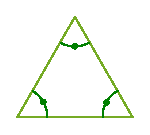
\includegraphics[width=.8\linewidth]{exoEnt1}
\item 
\includegraphics[width=.8\linewidth]{exoEnt2}
\item 
\includegraphics[width=.8\linewidth]{exoEnt3}
\item 
\includegraphics[width=.8\linewidth]{exoEnt4}
\end{colenumerate}
\end{exercice}



\begin{exercice}
Dans chaque cas, effectue un croquis puis construis la figure.
\begin{colenumerate}{1}
\item Trace un triangle $FIN$ rectangle en $F$ tel que $FI$ = 5 cm et $NF$ = 6 cm.
\item Trace un triangle $TRS$ rectangle en $S$ tel que $TS$ = 72 mm et $SR$ = 85 mm.
\item Construis un triangle $MNO$ équilatéral de côté 5 cm.
\item Construis un triangle isocèle $STU$ isocèle en $S$ tel que $ST$ = 58 mm et $TU$ = 32 mm.
\item Construis un triangle $ABC$ tel que $AB$ = 6 cm ; $BC$ = 5,2 cm et $CA$ = 42 mm.
\end{colenumerate}
\end{exercice}



\begin{exercice}[Médiatrices dans un triangle]
\begin{enumerate}
\item Construis un triangle $ABC$ tel que $AB$ = 5,7 cm, $AC$ = 5,3 cm et $BC$ = 7 cm.
\item Construis les médiatrices des segments $[AB]$ et $[CB]$. Note $O$ leur point d'intersection.
\item Construis la médiatrice du segment $[AC]$. Que constates‑tu ?
\item Trace le cercle de centre $O$ passant par $A$. Comment s'appelle ce cercle ?
\end{enumerate}
\end{exercice}



\begin{exercice}[Bissectrice dans un triangle]
\begin{enumerate}
\item Trace un triangle $UST$ tel que $UT$ = 6 cm ; $US$ = 10 cm et $ST$ = 14 cm.
\item Construis les bissectrices des angles $\widehat{UST}$, $\widehat{UTS}$ et $\widehat{TUS}$.

Que constates‑tu ?
\end{enumerate}
\end{exercice} 




\begin{exercice}
Dans les 6 cas suivants, détermine si la droite $d$ est :
\begin{enumerate}
\item une hauteur ;
\item une médiatrice ;
\item une bissectrice ;
\item une médiane.
\end{enumerate}

\begin{colenumerate}{3}
\item 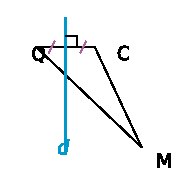
\includegraphics[width=.8\linewidth]{exoEnt5}
\item 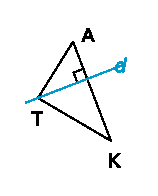
\includegraphics[width=.8\linewidth]{exoEnt6}
\item 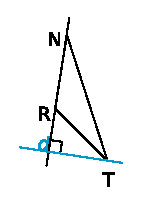
\includegraphics[width=.8\linewidth]{exoEnt7}
\item 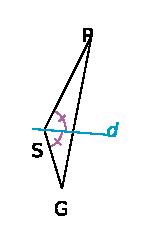
\includegraphics[width=.8\linewidth]{exoEnt8}
\item 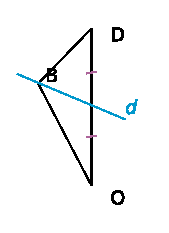
\includegraphics[width=.8\linewidth]{exoEnt9} 
\item 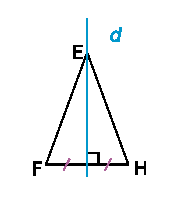
\includegraphics[width=.8\linewidth]{exoEnt10}
\end{colenumerate}
\end{exercice}




\begin{exercice}[Vocabulaire]
\begin{enumerate}
\item Construis un triangle $BOA$ tel que $BO$ = 5 cm, $OA$ = 7 cm et $AB$ = 8 cm. Trace la droite $d_1$ perpendiculaire à $[BO]$ et passant par $A$.
\item Trace la droite $d_2$ perpendiculaire au segment $[OA]$ et passant par son milieu.
\item Trace la droite $d_3$ qui coupe l'angle $\widehat{OBA}$ en deux angles égaux.
\item Trace la droite $d_4$ qui passe par $O$ et par le milieu de $[BA]$.
\item Détermine quelle(s) droite(s) représente(nt) la hauteur du triangle.
\item Détermine quelle(s) droite(s) représente(nt) une médiatrice.
\item Détermine quelle(s) droite(s) représente(nt) une bissectrice.
\item Détermine quelle(s) droite(s) représente(nt) une médiane.
\end{enumerate}
\end{exercice}




\begin{exercice}[Hauteurs d'un triangle]
Construis un triangle $BON$ tel que $BO$ = 68 mm, $BN$ = 62 mm et $NO$ = 45 mm.

Trace :
\begin{itemize}
\item en noir, la perpendiculaire à $(BN)$ passant par $O$ ;
\item en rouge, la perpendiculaire à $(NO)$ passant par $B$ ;
\item en vert, la perpendiculaire à $(BO)$ passant par $N$. Que remarques‑tu ?
\end{itemize}
\end{exercice}


\begin{exercice}[Hauteur (« relative à » ou « issue de »)]
\begin{enumerate}
\item Construis un triangle $AVE$ quelconque puis trace :
    \begin{itemize}
    \item en bleu, la hauteur issue du sommet $E$ ;
    \item en noir, la hauteur issue du sommet $A$ ;
    \item en rouge, la hauteur relative à $[AE]$.
    \end{itemize}
\item Observe ces trois hauteurs. Quelle remarque peux-tu faire ?
\end{enumerate}
\end{exercice}



\begin{exercice}[À l'intérieur ou pas ?]
\begin{enumerate}
\item Construis un triangle $DER$ ayant tous ses angles aigus. Trace les hauteurs de ce triangle.
\item Construis un triangle $NRV$ tel que $\widehat{NRV}$ soit un angle obtus. Trace les hauteurs de ce triangle.
\item Construis un triangle $GHT$ rectangle en $T$. Trace les hauteurs de ce triangle.
\item Observe les trois figures. Quelles remarques peux-tu faire ?
\end{enumerate}
\end{exercice}



\begin{exercice}[Vocabulaire] 
\begin{enumerate}
\item Construis un triangle $OA$. Trace la droite $(d_1)$ perpendiculaire à $[BO]$ et passant par $A$.
\item Trace la droite $(d_2)$ perpendiculaire au segment $[OA]$ et passant par son milieu.
\item Trace la droite $(d_3)$ qui coupe l'angle $\widehat{BOA}$ en deux angles égaux.
\item Trace la droite $(d_4)$ qui passe par $O$ et par le milieu de $[BA]$.
\item Reformule les questions précédentes en utilisant les mots : médiatrice, bissectrice, médiane et hauteur.
\end{enumerate}
\end{exercice}



\begin{exercice}[Cercles circonscrits]
Dans chaque cas, construis le triangle $LYS$ puis son cercle circonscrit.
\begin{enumerate}
\item $LS$ = 8 cm, $\widehat{YLS}$ = 65° et $\widehat{YSL}$ = 45°.
\item $LS$ = 4 cm, $LY$ = 5 cm et $\widehat{YLS}$ = 103°.
\item $LYS$ est isocèle en $L$ tel que $LY$ = 8 cm et $YS$ = 5,5 cm.
\item $LYS$ est un triangle équilatéral de côté 6 cm.
\end{enumerate}
\end{exercice}




\begin{exercice}[Sois malin !]
\begin{enumerate}
\item Construis un triangle $MEC$ tel que son cercle circonscrit ait un rayon de 5 cm.
\item Construis un triangle $RNB$ isocèle en $B$ avec $BN$ = 4 cm tel que son cercle circonscrit ait un rayon de 5 cm.
\end{enumerate}
\end{exercice}



\begin{exercice}[Cercle inscrit]
Dans chaque cas, construis le triangle $ABC$ puis son cercle inscrit.
\begin{enumerate}
\item $AC$ = 8 cm, $\widehat{BAC}$ = 60° et $\widehat{ACB}$ = 50°.
\item $AC$ = 10 cm, $AB$ = 8 cm et $\widehat{BAC}$ = 45°.
\item $ABC$ est isocèle en $A$ tel que $AB$ = 9 cm et $BC$ = 6 cm.
\item $ABC$ est un triangle équilatéral de côté 7,5 cm.
\end{enumerate}
\end{exercice}



\serie{Utiliser le vocabulaire associé aux angles}






\begin{exercice}
$\hat{a}$ et $\hat{b}$ sont deux angles complémentaires.

Calcule la mesure de $\hat{b}$ si :

$\hat{a}$ = 45°,\hfill%
$\hat{a}$ = 37°,\hfill%
$\hat{a}$ = 2°,\hfill%
$\hat{a}$ = 88,3°.  
\end{exercice}



\begin{exercice}
$\hat{x}$ et $\hat{y}$ sont deux angles supplémentaires.

Calcule la mesure de $\hat{y}$ si :

$\hat{x}$= 103°,\hfill%
$\hat{x}$= 95°,\hfill%
$\hat{x}$= 56°,\hfill%
$\hat{x}$= 0,3°.
\end{exercice}




\begin{exercice}
Indique si les angles proposés sont adjacents, complémentaires ou bien encore supplémentaires. Justifie tes réponses. 

\begin{center}
    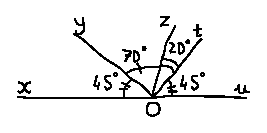
\includegraphics[width=.8\linewidth]{exoEnt11}
\end{center}

\begin{enumerate}
\item $\widehat{yOz}$ et $\widehat{zOt}$ ;
\item $\widehat{xOy}$ et $\widehat{yOu}$ ;
\item $\widehat{xOy}$ et $\widehat{tOu}$ ;
\item $\widehat{yOu}$ et $\widehat{tOu}$ ;
\item $\widehat{xOz}$ et $\widehat{zOt}$ ;
\item $\widehat{xOt}$ et $\widehat{uOt}$.
\end{enumerate}
\end{exercice}


\columnbreak
\begin{exercice}[Les deux font la paire]
Nomme, en justifiant, deux angles de la figure, codés ou non :
\begin{enumerate}
\item complémentaires et adjacents ;
\item complémentaires et non adjacents ;
\item supplémentaires et adjacents ;
\item supplémentaires et non adjacents ;
\item opposés par le sommet.
\end{enumerate}

\begin{center}
    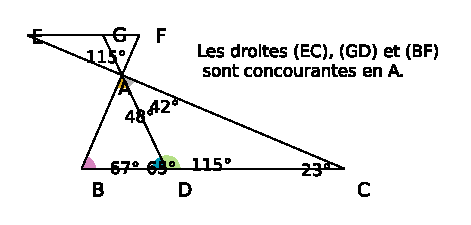
\includegraphics[width=\linewidth]{exoEnt12}
\end{center}

\end{exercice}




\begin{exercice}[Les angles inconnus]
\begin{enumerate}
\item Trouve la mesure de deux angles complémentaires, sachant que l'un d'eux est 8 fois plus grand que l'autre.
\item Trouve la mesure de deux angles supplémentaires, sachant que l'un d'eux est 9 fois plus petit que l'autre.
\end{enumerate}
\end{exercice}



\begin{exercice}[Des angles dynamiques...]
\begin{enumerate}
\item À l'aide du logiciel \emph{TracenPoche}, construis deux angles complémentaires et adjacents.
\item Propose une façon de procéder pour que ces angles restent adjacents, complémentaires et égaux à 45°, même quand on bouge les points.
\end{enumerate}
\end{exercice}



\begin{exercice}
Que peut-on dire des angles :

\begin{minipage}{.3\linewidth}
\begin{enumerate}
\item 1 et 3 ?
\item 1 et 5 ?
\item 3 et 5 ?
\item 1 et 4 ?
\item 4 et 6 ?
\item 3 et 7 ?
\end{enumerate}
\end{minipage}\hfill%
\begin{minipage}{.67\linewidth}
\centering
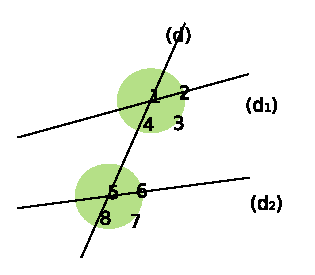
\includegraphics[width=\linewidth]{exoEnt13}
\end{minipage}
\end{exercice}




\begin{exercice}
Nomme deux angles de la figure et précise le nom de la sécante correspondante :
\begin{enumerate}
\item alternes-internes avec l'angle \no 3 ;
\item correspondants avec l'angle \no 10 ;
\item alternes-internes avec l'angle \no 13 ;
\item correspondants avec l'angle \no 7.
\end{enumerate}

\begin{center}
    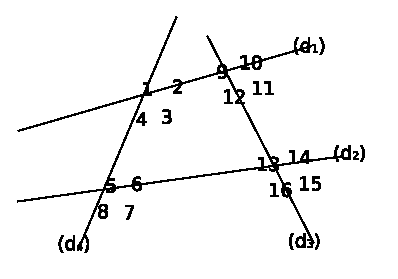
\includegraphics[width=.8\linewidth]{exoEnt14}
\end{center}

\end{exercice}



\begin{exercice}[Recherche de mesures d'angles]
\begin{enumerate}
\item Nomme deux paires d'angles de la figure :
    \begin{itemize}
    \item alternes-internes aigus ;
    \item alternes-internes de même mesure ;
    \item correspondants aigus ;
    \item supplémentaires et non adjacents.
    \end{itemize}
    
\begin{center}
    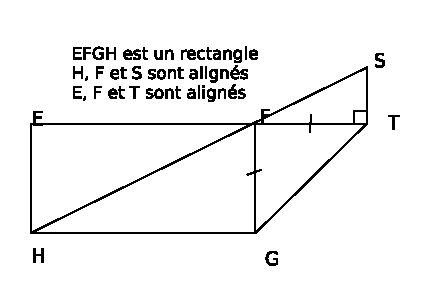
\includegraphics[width=.9\linewidth]{exoEnt15}
\end{center}

\item Sachant de plus que $\widehat{EFH}$ = 27°, calcule la mesure de l'angle $\widehat{SFT}$ puis celle de $\widehat{SFG}$.
\end{enumerate}
\end{exercice}

\columnbreak
\serie{Caractériser des droites parallèles par les angles}



\begin{exercice}
Dans chaque cas, dire si les droites $(d_1)$ et $(d_2)$ sont ou non parallèles et pourquoi.
\begin{center}
    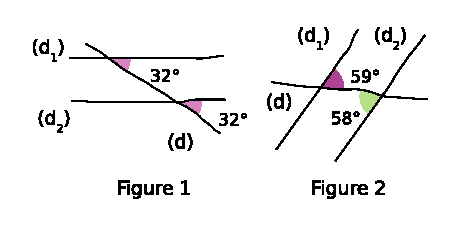
\includegraphics[width=.8\linewidth]{exoEnt16}
\end{center}
\end{exercice} 



\begin{exercice}[Le coup des équerres !]
Arnaud a placé ses deux équerres identiques sur la droite $(d)$ comme l'illustre le schéma ci-dessous.

\begin{center}
    
\includegraphics[width=.8\linewidth]{exoEnt17}
\end{center}

\begin{enumerate}
\item Il affirme que, de cette façon, il peut tracer des droites parallèles. Est-ce vrai et pourquoi ?
\item Quelles seraient les autres façons de positionner les équerres pour obtenir le même résultat ?
\end{enumerate}
\end{exercice} 



\begin{exercice}[Angles et droites parallèles]

\begin{center}
    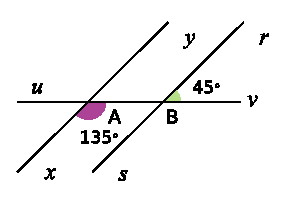
\includegraphics[width=.8\linewidth]{exoEnt18}
\end{center}

\begin{enumerate}
\item Calcule la mesure de l'angle $\widehat{uBr}$.
\item Les droites $(xy)$ et $(sr)$ sont-elles parallèles ? Justifie ta réponse.
\end{enumerate}
\end{exercice}



\columnbreak
\serie{Calculer des angles formés par des\\ droites parallèles}





\begin{exercice}[Parallèles ?]
Sur la figure ci-dessous, les angles $\widehat{BAE}$ et $\widehat{FEO}$ sont égaux à 58°.

\begin{center}
    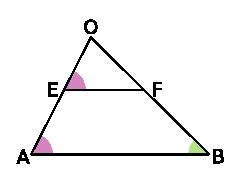
\includegraphics[width=.7\linewidth]{exoEnt19}
\end{center}

\begin{enumerate}
\item Que peux-tu dire des droites $(EF)$ et $(AB)$ ? Justifie ta réponse.
\item On sait de plus que la mesure de l'angle $\widehat{FBA}$ est 45°. Déduis-en la mesure de l'angle $\widehat{OFE}$. Justifie ta réponse.
\end{enumerate}
\end{exercice}


\begin{exercice}[Droites parallèles]

\begin{center}
    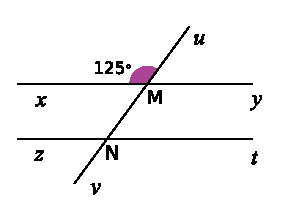
\includegraphics[width=.7\linewidth]{exoEnt20}
\end{center}

Sur la figure ci-dessus, les droites $(xy)$ et $(zt)$ sont parallèles. L'angle $\widehat{xMu}$ vaut 125°.
\begin{enumerate}
\item Donne la mesure de l'angle $\widehat{vMy}$. Justifie ta réponse.
\item Donne d'autres angles dont la mesure est de 125°. Justifie ta réponse.
\end{enumerate}
\end{exercice}

\newpage
\begin{exercice}[Angles supplémentaires]
                        
\begin{center}
    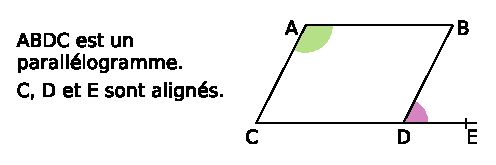
\includegraphics[width=\linewidth]{exoEnt21}
\end{center}
                                 
\begin{enumerate}
\item Justifie que les angles $\widehat{BAC}$ et $\widehat{BDC}$ sont de même mesure.
\item Que dire des angles $\widehat{BDC}$ et $\widehat{BDE}$ ? Pourquoi ? Justifie alors que les deux angles marqués sont supplémentaires.
\end{enumerate}
\end{exercice}

\columnbreak
\begin{exercice}[Zigzag]

\begin{center}
    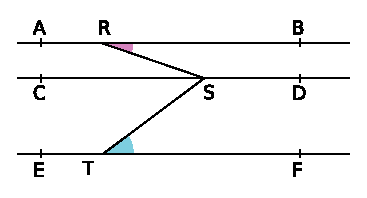
\includegraphics[width=.8\linewidth]{exoEnt22}
\end{center}

Sur la figure ci-dessus :
\begin{itemize}
    \item les droites $(AB)$, $(CD)$ et $(EF)$ sont parallèles ;
    \item $R$ est un point de la droite $(AB)$, $S$ est un point de la droite $(CD)$ et $T$ est un point de la droite $(EF)$ tels que : $\widehat{BRS}$ = 20° et $\widehat{RST}$ = 57°.
\end{itemize}

Calcule la mesure de l'angle $\widehat{STF}$.
\end{exercice}


\begin{exercice}
Construis à l'aide de \emph{TracenPoche} un quadrilatère $EFGH$ ayant deux angles droits, en $E$ et en $G$.
\begin{enumerate}
\item Affiche la mesure des angles $\widehat{EFG}$ et $\widehat{EHG}$. Que remarques-tu ?
\item Trace le segment $[FH]$. En raisonnant dans les triangles $EFH$ et $FHG$, démontre que $\widehat{EFG}$ et $\widehat{EHG}$ sont supplémentaires.
\end{enumerate}
\end{exercice}
